Particle samples of each of the four aerosol types used in this study were collected and imaged by SEM. Samples were collected from size-classified aerosol at the same mobility diameters, as used for optical measurements: 240 nm for soot and agglomerated CB, 150 nm for nigrosin and compact CB. Soot aggregates (Figure \ref{fig:sem}a) are highly fractal whereas nigrosin particles are fully spherical (Figure \ref{fig:sem}b). Morphology of the atomized CB strongly depends on the aerosol dilution approach. The two types of dilution configuration used in this study are illustrated in Figure \ref{fig:system}. If droplets produced upon atomization are immediately diluted with dry air, CB aggregates are compact and nearly spherical (Figure \ref{fig:sem}d). However, if the generated aqueous aerosol is not diluted immediately (Figure \ref{fig:system}b), droplets coalesce and, after drying, produce semi-fractal aggregates made of multiple compact units (Figure \ref{fig:sem}c). Adjusting aerosol residence time before dilution with dry air (Figure \ref{fig:system}c) can be used to vary the morphology of CB from fully compact particles to agglomerates of compact particles. An important feature observed in most images, and especially prominent in the image of nigrosin, is the presence of larger multiply charged particles. For instance, for nigrosin, in addition to the most numerous singly charged 147 nm particles (as measured from the SEM image shown in Figure \ref{fig:sem}b), we observed the presence of fewer numbers of larger doubly charged (235 nm) and even triply charged (294 nm) particles. Additionally, nigrosin shows the presence of doublets among the 147 nm particles, which were formed by coalescense of dry particles. 

Particle morphology can be described quantitatively using different metrics, such as convexity and mass-mobility scaling exponent \citep{RN69}. Average convexities of particles in Figure \ref{fig:sem} were found to be (a) $0.61\pm 0.01$, (b) $0.96\pm 0.01$, (c) $0.78\pm 0.01$, and (d) $0.90\pm 0.01$, high values for more compact particles in agreement with visual observations.

\begin{figure}[htp]
\centering
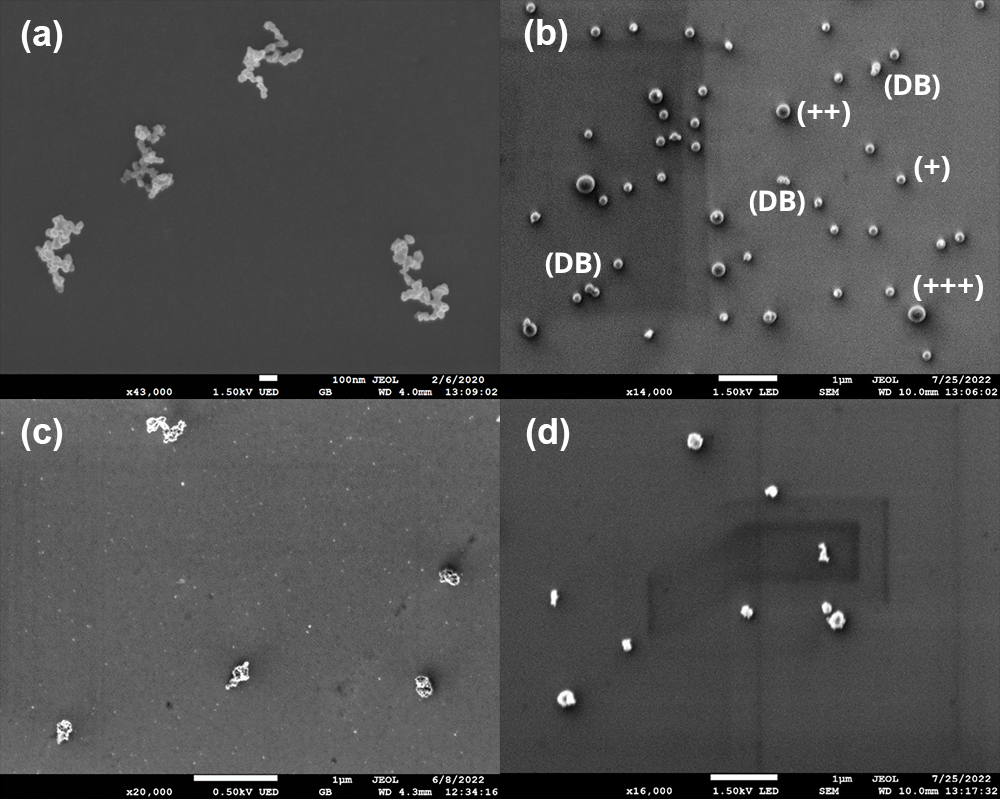
\includegraphics[width=\textwidth]{fig_sem.png}
\caption{SEM images of: (a) flame-generated soot, (b) nigrosin, (c) agglomerated CB, and (d) compact CB. In the image for nigrosin, (+), (++), and (+++) mark the singly, double, and triply charged particles with diameters of 147, 235, and 294 nm, respectively, and (DB) marks doublets from coagulation. Mobility diameters used to classify these particles: (a) 240 nm, (b) 150 nm, (c) 240 nm, and (d) 150 nm}
\label{fig:sem}
\end{figure}

The mass-mobility exponent can be determined from the dependence of the particle mass on the electrical mobility diameter (Equation \ref{eq:mass_prop}), where for spherical particles, mass is proportional to the cube of diameter. This relationship can be written in relative form, where the electrical mobility diameter is normalized by a reference electrical mobility diameter, and mass is normalized by mass of particles of that reference electrical mobility diameter, allowing us to eliminate the proportionality constant (Equation \ref{eq:mass_mobility}).
\begin{equation}
    \label{eq:mass_prop}
    m\propto D^3
\end{equation}
\begin{equation}
    \label{eq:mass_mobility}
    \frac{m}{m_{\rm ref}}=\left(\frac{D}{D_{\rm ref}}\right)^\varepsilon
\end{equation}
Particle deviation from a spherical geometry causes the exponent in Equation \ref{eq:mass_mobility} to deviate from 3, while the overall power law dependence remains valid. Hence, we can define a general mass-mobility law, where $\varepsilon$ is mass-mobility exponent, which is similar, but not equivalent to $D_f$.

To determine compactness, mass of particles of different electrical mobility diameters can be measured and $\varepsilon$ can be calculated by fitting the data to Equation \ref{eq:mass_mobility}. Such mass-mobility measurements were performed for the four aerosol types mentioned above and also for PSL, using 150 nm - 350 nm electrical mobility diameter particles (Figure \ref{fig:mass_mobility}). Perfectly spherical PSL particles produced mass mobility exponent of 3.00. Nigrosin particles, albeit spherical, produced  somewhat lower $\varepsilon$ approaching 2.95. Soot aggregates were highly fractal, with a mass-mobility exponent of 2.36. Carbon black particles fell between highly fractal soot and spherical nigrosin, with the mass-mobility exponent for compact CB closer to nigrosin (2.88) and that of agglomerated CB closer to soot (2.68).

\begin{figure}[htp]
    \centering
    \begin{tikzpicture}
    \begin{loglogaxis}[
    xlabel={$D,\ \rm nm$},
    ylabel={$m,\ \rm fg$},
    legend pos=north west,
    legend cell align={left},
    ymax=500,
    xtick={150,240,350},
    xticklabels={$150$,$240$,$350$}
    ]
        \addplot [only marks,color=tab_purple,mark=star] table {plots/mass_mobility_absolute/psl.txt};
        \addlegendentry{PSL, $\varepsilon=3.00$}
        % 1.0000    0.4980    0.0549
        \addplot [only marks,color=tab_orange,mark=square*] table {plots/mass_mobility_absolute/nigrosin.txt};
        \addlegendentry{Nigrosin, $\varepsilon=2.95$}
        \addplot [only marks,color=tab_grey,mark=triangle*] table {plots/mass_mobility_absolute/cb_cmp.txt};
        \addlegendentry{CB\textsubscript{cmp}, $\varepsilon=2.88$}
        \addplot [only marks,color=tab_red,mark=diamond*] table {plots/mass_mobility_absolute/cb_agg.txt};
        \addlegendentry{CB\textsubscript{agg}, $\varepsilon=2.68$}
        \addplot [only marks,color=tab_blue,mark=otimes*] table {plots/mass_mobility_absolute/soot.txt};
        \addlegendentry{Soot, $\varepsilon=2.36$}
        % PSL fit
        \addplot [domain=150:350,no markers,color=tab_purple] {5.386995e-07*x^3.004721};
        % Nigrosin fit
        \addplot [domain=150:350,no markers,color=tab_orange] {9.701697e-07*x^2.948992};
        % CB200_cmp fit
        \addplot [domain=150:350,no markers,color=tab_grey] {6.617110e-07*x^2.880935};
        % CB200_agg fit
        \addplot [domain=150:350,no markers,color=tab_red] {1.996164e-06*x^2.684836};
        % Soot fit
        \addplot [domain=150:350,no markers,color=tab_blue] {5.483814e-06*x^2.363773};
    \end{loglogaxis}
    \end{tikzpicture}
    \caption{Dependence of mass on the electrical mobility diameter for bare particles of different types. Listed mass mobility exponents ($\varepsilon$) are obtained from exponential fits.}
    \label{fig:mass_mobility}
\end{figure}

Mass-mobility measurements support the trend in convexities determined from SEM images and provide an alternative quantitative way to compare the morphology of different particle types. It is interesting to note that $\varepsilon$ for nigrosin is 2.95 and not exactly 3.00, as measured for PSL. This deviation from the mass-mobility exponent of 3.00, as expected for spherical particles, can be due to a slight decrease in particle effective density with increasing mobility diameter. The mass distributions of nigrosin particles in Figure S2 exhibit a tail towards lower masses as the mobility diameter increases, confirming this observation.
